\chapter{Evaluation}
\label{chap:evaluation}

To evaluate the quality of the algorithm proposed in chapter
\ref{chap:gradient-free}, I have implemented a proof-of-concept optimizer.
I will compare \texttt{Crotosolve} to several other optimizers frequently used
in QML by creating a loss curve benchmark for all optimizers.
The benchmark features parameterizable quantum circuits with various degrees of
expressibility and from various research applications.

\section{Proof of Concept}
To put the approach proposed in chapter \ref{chap:gradient-free} to test,
I have implemented a proof-of-concept application with PennyLane
\cite{bergholm_pennylane_2022}.
PennyLane is a popular quantum computing SDK with extensive documentation and a
library of readily implemented optimizers \cite{unitary_fund_team_results_2022}.
Particularly, PennyLane is currently the only quantum SDK to implement the
\texttt{Rotosolve} optimizer, to which I want to compare my \texttt{Crotosolve}
optimizer in section \ref{sec:optimizer-comparison}.

Like the \texttt{Rotosolve} algorithm, \texttt{Crotosolve} optimizes each
parameter individually.
For each parameter corresponding to a controlled rotational Pauli gate,
\texttt{Crotosolve} first reconstructs the univariate cost function (see section
\ref{sec:constants}) and then use a numerical optimizer to find the minimizing
parameter value (see section \ref{sec:minimization}).
Each parameter corresponding to an uncontrolled rotational Pauli gate can be
optimized following the exact approach presented by Ostaszewski et al.
\cite{ostaszewski_structure_2021}.
The pseudocode for this algorithm is stated in algorithm \ref{alg:crotosolve}.

\begin{algorithm}
    \caption{The \texttt{Crotosolve} algorithm updates parameter individually}
    \label{alg:crotosolve}
    %
    \SetKwFunction{ReconstructCrp}{ReconstructCrp}
    \SetKwFunction{RotosolveUpdate}{RotosolveUpdate}
    \SetKwFunction{MakeUnivariate}{MakeUnivariate}
    %
    \KwData{$prev\_params \in \mathbb R^n$, $circuit$}
    \KwResult{$params \in \mathbb R^n$}
    \BlankLine
    $params \gets copy(prev\_params)$\;
    \For{$p \gets 1$ \KwTo $n$}{
        $uni \gets $ \MakeUnivariate{$circuit$, $params$, $p$}\;
        \eIf{$p$ belongs to controlled gate}{
            $recon \gets $ \ReconstructCrp{$uni$} \Comment*[r]{see section \ref{sec:constants}}
            $next\_params[p] \gets \underset{x \in [0, 4\pi]}{\operatorname{argmin}}\, recon(x)$ \Comment*[r]{using numerical minimizer}
        }{
            $next\_params[p] \gets $ \RotosolveUpdate{$uni$}\;
        }
    }
\end{algorithm}

This algorithm allows the optimization of parameterized quantum circuits where
all parameterized gates are either RP or CRP gates.
Furthermore, it is assumed that all gate parameters are used without
preprocessing (e.g., having a $RP(x^2)$ gate for a parameter $x$) in only a
single gate.
The algorithm needs to know which parameters belong to CRP and which belong to
RP gates.
Technically, the optimization approach presented for CRP gates could also be
used for RP gates since a CRP gate's loss function structure is a generalization
of an RP gate's loss function structure.
However, using the CRP optimization approach for RP gates would double the
number of circuit evaluations required to reconstruct its loss function.
While it is trivial to see if a parameter is used in a CRP or RP gate on paper,
looking up this relationship in a given PennyLane circuit is non-trivial,
although certainly possible.
% TODO: really?
Thus, the proof-of-concept implementation always stores the RP and CRP gate
parameters as separate arrays.

\section{Optimizer comparison}
\label{sec:optimizer-comparison}
% TODO: rename, check usages

I will examine \texttt{Crotosolve}'s performance by comparing its loss curve
with the loss curves of other optimizers frequently used in the field of QML.
This comparison includes the Gradient Descent family of optimizers, namely
standard gradient descent with a fixed learning rate, % TODO: cite! and isnt this really stochastic GD?
\texttt{Adam} \cite{kingma_adam_2017} and
\texttt{Adagrad} \cite{duchi_adaptive_2011}.
Additionally, I will test my \texttt{Crotosolve} implementation against
PennyLane's implementation of the \texttt{Rotosolve} algorithm
\cite{ostaszewski_structure_2021,bergholm_pennylane_2022}, which is extended by
Wierichs' paper on ``\emph{\citefield{wierichs_general_2022}{title}}'' to
support further types of gates \cite{wierichs_general_2022}.

To get meaningful results, I chose to run these optimizers on well-known and
widely-used quantum circuits.
Specifically, I use the set of circuit templates presented in a paper on
``Expressibility and Entangling Capability [...]'' metrics by Sukin Sim et al.
\cite{sim_expressibility_2019}.
As shown in this paper, these circuits have various degrees of expressibility
and entangling capability. % TODO why is that good
% TODO mention that this set of circuits has also been used as a benchmark in
%      other cases

The optimizers are compared through loss curves generated from exemplary
circuits.
These loss curves are recorded with respect to the number of circuit
evaluations, even though it would be more common in classical machine learning
to use the number of iterations or taken time instead of the evaluations.
The time taken to run these quantum circuits on classical hardware using
state-vector simulation is hardly representative of the actual runtime on
quantum devices since this simulation task is proven to be inefficient.
% TODO: cite!
Additionally, the optimizers benefit to varying degrees from optimizations made
in the simulation.
For example, gradient-based optimizers benefit from PennyLane's gradient
evaluation optimization, which is unavailable on real quantum hardware.
% TODO: cite!
Meanwhile, gradient-free optimizers like \texttt{Crotosolve} and
\texttt{Rotosolve} cannot take advantage of these simulation tricks.
On the other hand, iterations put \texttt{Crotosolve} and \texttt{Rotosolve} in
favor since each of their iterations encompasses many univariate optimizations.
Circuit evaluations, however, are proportional to the execution time on real
quantum hardware as long as the classical work required between evaluations is
negligible.

\begin{figure}
    \label{fig:avg-loss-curve}
    \centering
    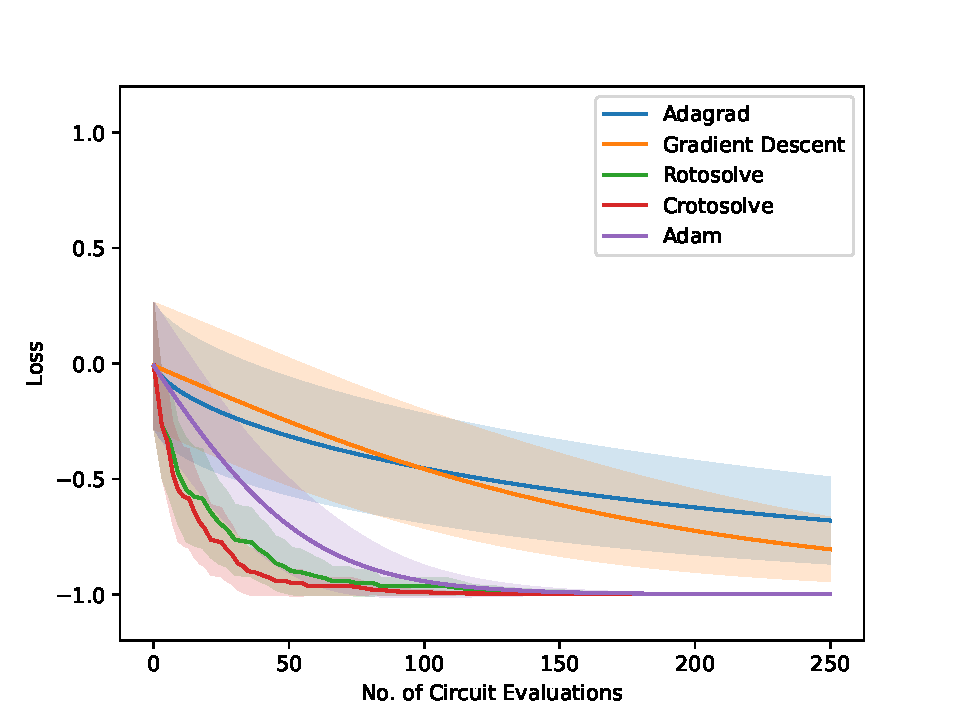
\includegraphics[width=0.7\textwidth]{loss-curve_sim11_4x3.pdf}
    \caption{Various optimizers minimize the expectation of circuit 11 from
        \cite{sim_expressibility_2019} with four qubits and three layers.
        Full lines show the average loss curve.
        Transparent areas show the error, which is the average $\pm$ its
        standard deviation.}
\end{figure}

I have generated many random initial parameter values for each circuit to
reduce statistical noise through averaging.
Each pair of circuits and parameter values is run with each optimizer to
record the loss curve of its optimization as a result.
These results are then aggregated in average loss curves for each pair of
circuits and optimizers.

Figure \ref{fig:avg-loss-curve} shows the average loss curves for each
optimizer on circuit 11.
I have selected this chart as it shows all the key characteristics described in
the following, but the charts for all other evaluated circuits can be found in
appendix \ref{chap:appendix}.
Furthermore, the circuit and initial values data for all evaluated circuits, as
well as the recorded loss curve data is available on GitHub \cite{crotosolve}.

% TODO describe the device this has been run on

\subsubsection*{Results}

\texttt{Crotosolve}'s loss curve generally is very similar to
\texttt{Rotosolve}'s loss curve, although consistently below.
For RP gates, this is easy to explain since both algorithms are identical.
For CRP gates, both algorithms use the same strategy, although different methods
to achieve their common goal.
PennyLane's implementation of the \texttt{Rotosolve} algorithm proposed by
Ostaszewski et al. is augmented with the work of Wierichs et al.
\cite{ostaszewski_structure_2021,wierichs_general_2022,bergholm_pennylane_2022}.
Wierichs' work allows the algorithm to reconstruct univariate loss functions
from almost any quantum circuit through a discrete Fourier series transform.
While both \texttt{Crotosolve} and \texttt{Rotosolve} cache an evaluation value
between RP gate optimization steps, only \texttt{Crotosolve} does so for
CRP gates too.
This enhanced caching ensures that \texttt{Crotosolve}'s loss curve is always
slightly better than \texttt{Rotosolve}'s.

Additionally, \texttt{Rotosolve} has to compute the circuit parameter
frequencies to reconstruct the univariate loss curves.
It is sufficient to compute these frequencies once before the first
\texttt{Rotosolve} iteration.

Figure X shows an example loss curve chart, featuring the average results of all
optimizers for a random circuit Y instance. % TODO mention actual numbers

% TODO actually put them in the appendix
% TODO this sounds a lot like results were selected, emphasis should be on this
%      chart showing ALL characterists that can also be found in other charts

Comparison to gradient-based optimizers: 



\subsubsection*{Discussion}

\begin{itemize}
    \item mention complexity, compare number of evaluations
    \item comment on generality/limitations: parameter independence, universal gate sets, ...
\end{itemize}

\section{Outline}
\begin{itemize}
    \item
        Evaluate the accuracy of the model, the number of steps in the
        optimization loop and the number of circuit evaluations
        \cite{wendenius_gradient-free_2023,ostaszewski_structure_2021}.
    \item
        Compare the results with the performance of other established
        optimizers (e.g., Adam \cite{kingma_adam_2017}, Gradient Descent and
        Quantum Natural Gradient \cite{stokes_quantum_2020}) as well as the
        \emph{Sine Exact} and \emph{Sine Iterative} variants proposed in
        \cite{wendenius_gradient-free_2023}.
        % TODO: sources for other optimizers
        For this purpose, evaluate at least the circuits from
        \cite{sim_expressibility_2019} that were also evaluated in the
        Wendenius et al. paper \cite{wendenius_gradient-free_2023}.
        % TODO: more circuits to evaluate? eileen might have access to
        %       something...
    \item
        Think about the effects of barren plateaus on this optimizer.
        % TODO: do think about this and come up with a concrete task!
        % TODO: cite barren plateaus
\end{itemize}
